\documentclass{beamer}

\usepackage[space]{xeCJK}

% Overleaf版本
%\setCJKmainfont{Noto Serif CJK SC}
%\setCJKsansfont{Noto Sans CJK SC}
%\setCJKmonofont{Noto Sans Mono CJK SC}

% 本地编译器
\setCJKmainfont{楷体}[BoldFont=黑体]

\mode<presentation>
{
  \usetheme{CambridgeUS}
  \setbeamercovered{transparent}
}

\usepackage[english]{babel}
\usepackage{times}
\usepackage[T1]{fontenc} 
\usepackage{amsmath}
\usepackage{xcolor}
\usepackage[doipre={doi:~}]{uri}
\urlstyle{same}

\newcommand{\linespace}{\vskip 0.25cm}
\definecolor{MyForestGreen}{rgb}{0,0.7,0} 
\newcommand{\tableemph}[1]{{#1}}
\newcommand{\tablewin}[1]{\tableemph{#1}}
\newcommand{\tablemid}[1]{\tableemph{#1}}
\newcommand{\tablelose}[1]{\tableemph{#1}}

\definecolor{MyLightGray}{rgb}{0.6,0.6,0.6}
\newcommand{\tabletie}[1]{\color{MyLightGray} {#1}}

%\setbeamercolor*{palette tertiary}{bg=black}
\setbeamercolor{frametitle}{fg=black,bg=black!20}
\setbeamercolor{section in head/foot}{bg=black}
\setbeamercolor{author in head/foot}{bg=black}
\setbeamercolor{date in head/foot}{fg=black}
\setbeamercolor{title in head/foot}{fg=black} 
\setbeamercolor{institute in head/foot}{fg=black} 
\setbeamercolor*{subsection in head/foot}{fg=black}
\setbeamercolor*{title}{fg=black}
% \setbeamercolor*{title}{fg=white, bg=black}


%%%%%%%%%%%%%%%%%%%%%%%%%%%%%%%%%%%%%%%%%%%%%%%%%%%%%%%%%%%%
%%%%%%%%%%%%%%%%%%%%%%%%%%%%%%%%%%%%%%%%%%%%%%%%%%%%%%%%%%%%
\title[\textbf{学术报告}]{TSE(3)\textbf{上自主机动星群在小天体悬停任务中的\\几乎全局稳定方案及其离散化}}


\author[\textbf{雷~锋}]{雷~锋}


\institute[]
{
  哈尔滨工业大学  航天学院\\
  \linespace
  某某技术研究所 \\
}


\date{2023年2月31日}

\AtBeginSection[]
{
  \begin{frame}<beamer>
    \frametitle{Outline}
    \tableofcontents[currentsection, hideothersubsections]
  \end{frame}
}

%%%%%%%%%%%%%%%%%%%%%%%%%%%%%%%%%%%%%%%%%%%%%%%%%%%%%%%%%%%%
%%%%%%%%%%%%%%%%%%%%%%%%%%%%%%%%%%%%%%%%%%%%%%%%%%%%%%%%%%%%
\begin{document}

\begin{frame}
  \titlepage
\end{frame}


\section*{\textbf{概述}}

\subsection*{\textbf{前言}}

\begin{frame}
  \frametitle{\textbf{前言}}
  
  \begin{columns}
  \begin{column}{0.6\textwidth}
  \begin{itemize}
  	\item Developmental plasticity: a powerful source of flexibility in biology
	\item Most EC \& GP systems don't have a developmental phase
	\item Even fewer allow for plasticity during development
	\item N-gram GP has natural developmental phase
	\item Can we add plasticity?
  \end{itemize}
  \end{column}
  \begin{column}{0.4\textwidth}
   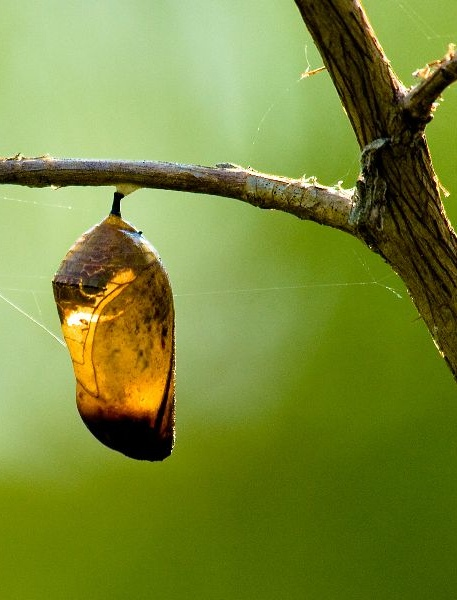
\includegraphics[width=0.95\textwidth]{Fig/FigA.jpg}
       \\
    \only{\tiny{Bluedrakon \\ \url{http://tr.im/pWUi} }}
  \end{column}
  \end{columns}
\end{frame}

\subsection*{\textbf{目录}}

\begin{frame}
  \frametitle{\textbf{目录}}
  \tableofcontents[hideallsubsections]
\end{frame}

\section[\textbf{帝皇的崛起}]{\textbf{帝皇的崛起}}

\subsection{\textbf{贯穿银河的大远征}}

\begin{frame}
  \frametitle{\textbf{贯穿银河的大远征}}
  
  \begin{columns}
  \begin{column}{.65\textwidth}
	让人类再次伟大!

\linespace

我来!我见!我征服!

\linespace
  
何为忠诚?何为背叛?大叛乱的萌芽

\linespace
  
普罗斯佩罗之焚
\linespace
  
考斯之战与暗影远征
  \end{column}
  \begin{column}{.35\textwidth}
    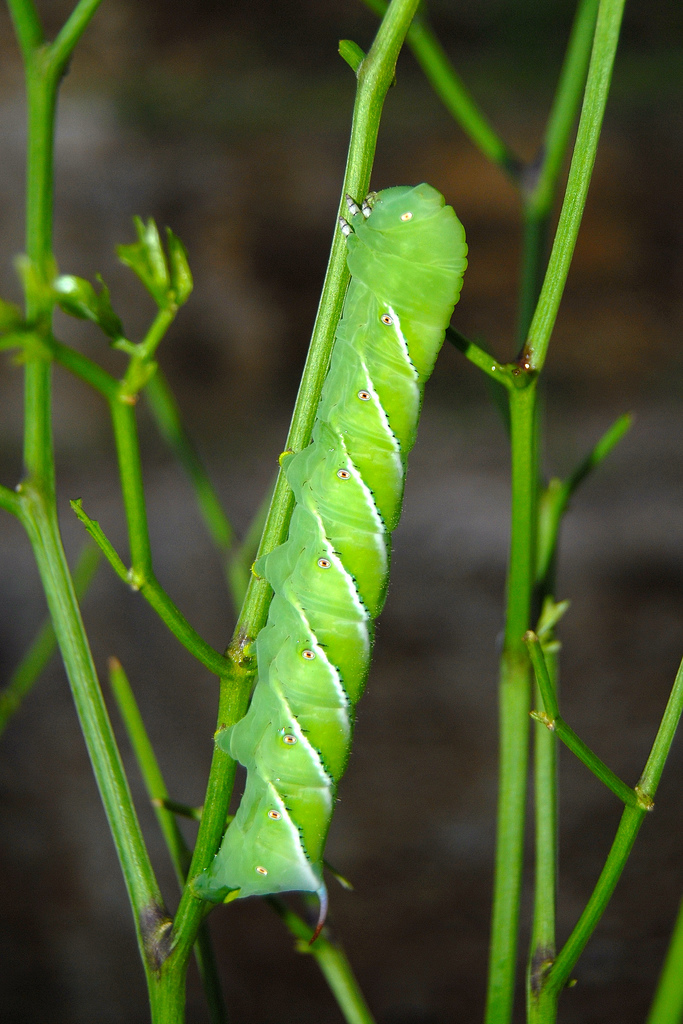
\includegraphics[width=.95\textwidth]{Fig/FigB.jpg}
    \\
    \tiny{Sam Fraser-Smith \\ \textcolor{blue}{\url{http://tr.im/pq7l}} }
  \end{column}
  \end{columns}

\end{frame}

\subsection{\textbf{荷鲁斯之乱}}

\begin{frame}
	\frametitle{\textbf{荷鲁斯之乱}}
	
	Most EC systems have no (or trivial) developmental processes.
	\begin{itemize}
		\item Therefore can't have developmental plasticity
	\end{itemize}
	
	\linespace
	
	There are important exceptions.  In GP, e.g.:
	\begin{itemize}
		\item Cellular encoding
		\item Many grammar-based systems
		\item DTAG3P
	\end{itemize}
	
	\linespace 
	
	These remain, however, the exception rather than the rule.
	
	\linespace
	
	N-gram GP has natural developmental process, so a good candidate for adding developmental plasticity.
\end{frame}

\begin{frame}
	\frametitle{\textbf{极限战士与考斯之战}}
	
	\begin{columns}
	\begin{column}{0.45\textwidth}
	N-gram GP uses a \emph{probability table} to store likelihood of a triple of instructions appearing in a program:
	\[ Pr\{ x_i \rightarrow x_{i+1} \rightarrow x_{i+2} \}. \]
				
		Given pair of instructions $(x_i, x_{i+1})$, this table gives us the probability distribution for the subsequent instruction $x_{i+2}$.
	\end{column}
	\begin{column}{0.55\textwidth}
	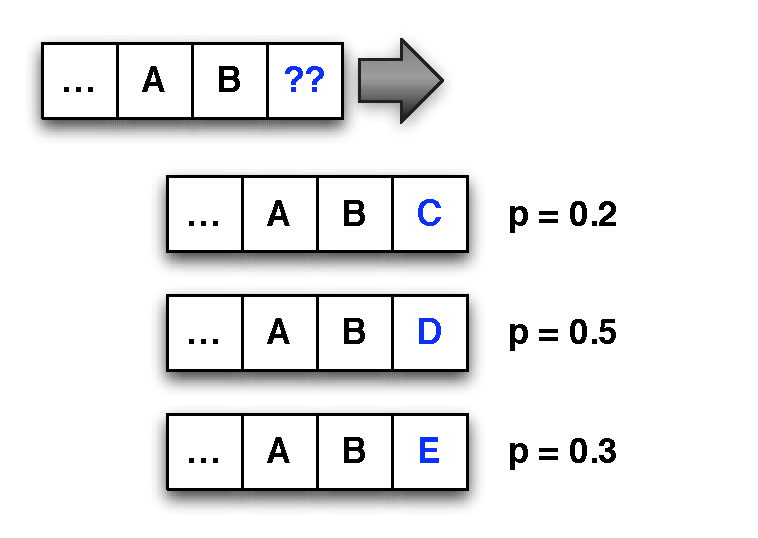
\includegraphics[width=\textwidth]{Fig/FigC.pdf}
	\end{column}
	\end{columns}
\end{frame}

\section[Results]{Results}

\subsection[Empirical results]{Empirical comparison of IFD, N-gram GP, and standard GP}

\begin{frame}
  \frametitle{Empirical comparison of IFD, N-gram GP, \& TinyGP}
  
  \begin{columns}[t]
  \begin{column}{0.45\textwidth}
  Compare IFD, regular N-gram GP, and standard sub-tree XO GP (TinyGP)
  \linespace
  \begin{itemize}
	\item 11 different symbolic regression problems
	\item 100 independent runs for each system + problem + parameter set
	\item Various parameter settings (e.g., different block sizes)
  \end{itemize}
  \end{column}

  \begin{column}{0.45\textwidth}
  2 register machine with $+, -, \times$, protected division, and swap
  
  \linespace
  
  Normalize the clock:
  \begin{itemize}
  	\item Count instruction executions
	\item Allow 50M instruction evaluations per run
	\item Store machine state so only new block has to be executed in IFD
  \end{itemize}
  
  \end{column}
  \end{columns}
\end{frame}

\begin{frame}
  \frametitle{Success rates on 11 test problems}
  
\begin{center}
\begin{tabular}{llrrr}
	& & \multicolumn{3}{c}{\emph{Successes out of 100 runs}} \\
	\textbf{Label} & \textbf{Function} & \textbf{TinyGP} & \textbf{N-gram} & \textbf{IFD} \\ \hline
	\tabletie{P1} & \tabletie{$x + x^2 + x^3 + x^4 + x^5$} & \tabletie{100} & \tabletie{100} & \tabletie{100} \\
	\tabletie{P2} & \tabletie{$-x-2x^2+x^3$} & \tabletie{100} & \tabletie{100} & \tabletie{100} \\
	P3 & $1.009 + 1.419x + x^2$ & \tablewin{100} & \tablelose{61} & \tablewin{100} \\
	\tabletie{P4} & \tabletie{$6+x^2+3x^3+8x^5$} & \tabletie{0} & \tabletie{0} & \tabletie{0} \\ \hline
	\tabletie{P5} & \tabletie{$6$} & \tabletie{100} & \tabletie{100} & \tabletie{100} \\ % P4d0f
	P6 & $6+x^2$ & \tablewin{100} & \tablelose{10} & \tablewin{94} \\ % P4d2f
	P7 & $6 + x^2 + 3 x^3$ & \tablewin{85} & \tablelose{0} & \tablelose{1} \\ \hline % P4d3f
	\tabletie{P8} & \tabletie{$8x^5$} & \tabletie{100} & \tabletie{100} & \tabletie{100} \\ % P4d5b
	P9 & $3x^3+8x^5$ & \tablelose{22} & \tablemid{55} & \tablewin{100} \\ % P4d3b
	P10 & $x^2+3x^3+8x^5$ & \tablewin{100} & \tablelose{7} & \tablemid{80} \\ \hline % P4d2b
	Sine & $sin(x)$ & \tablelose{0} & \tablelose{1} & \tablewin{63} \\ \hline
\end{tabular}
\end{center}
\end{frame}

\begin{frame}
\frametitle{IFD wins either way}

\begin{columns}
\begin{column}{0.6\textwidth}

\begin{itemize}
	\item IFD generates low-error individuals from tables evolved with IFD \textbf{and without IFD}.
	\linespace
	\item IFD's local search is valuable in all phases of the process, even if it wasn't used previously.
	\linespace
	\item N-gram GP isn't able to work effectively with the more complex probability tables that IFD generates.
\end{itemize}
\end{column}

\begin{column}{0.02\textwidth}
\end{column}

\begin{column}{0.5\textwidth}

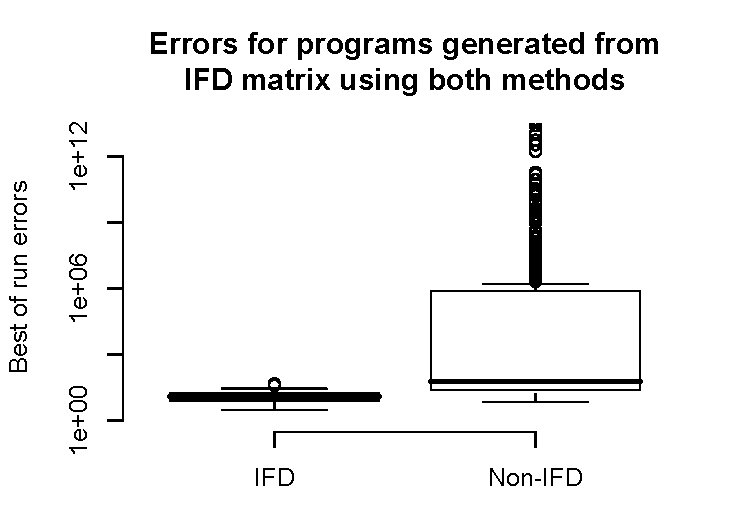
\includegraphics[width=0.915\textwidth]{Fig/FigD.pdf}

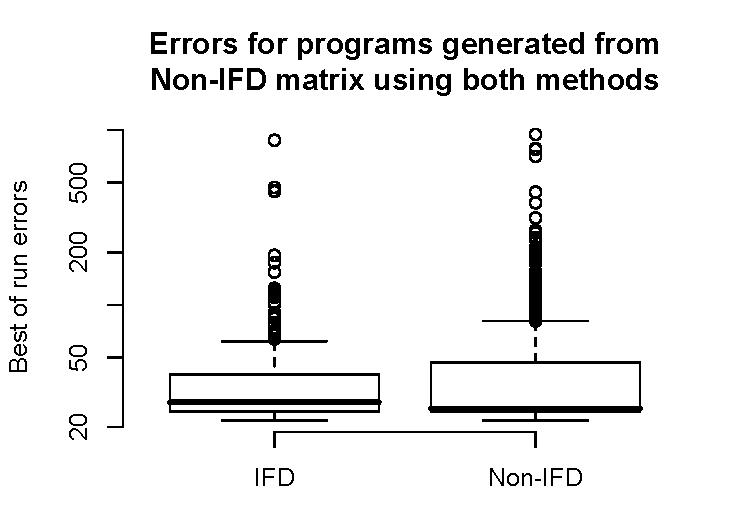
\includegraphics[width=0.915\textwidth]{Fig/FigE.pdf}

\end{column}
\end{columns}

\end{frame}

\subsection[Modularity]{Modularity and repeated structures in IFD}

\begin{frame}
  \frametitle{Structural differences and modularity}
  
  Standard N-gram GP tends to converge to a small set of loops with high probability edges.

  \begin{center}
  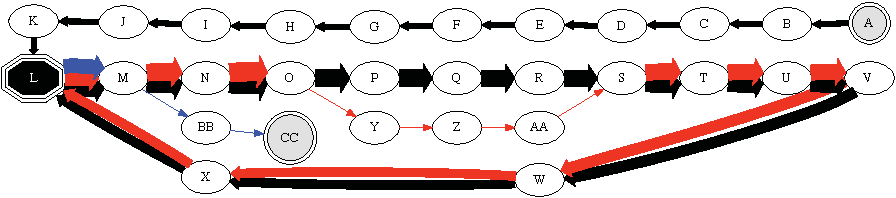
\includegraphics[width=0.8\textwidth]{Fig/FigF.pdf}
  \end{center}
  
      With IFD there is less convergence, more variety and complexity in the modular structure, \& greater use of low probability edges.
  
  \begin{center}
    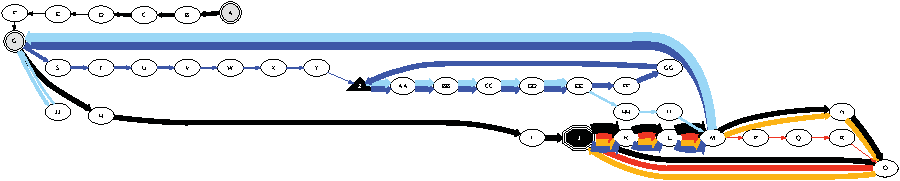
\includegraphics[width=\textwidth]{Fig/FigG.pdf}
    \end{center}

\end{frame}

\section[Conclusions]{Conclusions}

\begin{frame}
\frametitle{Conclusions}

\begin{itemize}
  \item Added developmental plasticity to N-gram GP using Incremental Fitness-based Development (IFD).
\end{itemize}

\begin{itemize}
  \item IFD consistently improved N-gram GP performance on suite of test problems.
  
  \linespace
  
  \item ``Knocking out'' IFD shows it's valuable in all phases, even if it wasn't used earlier in a run.

  \linespace
  
  \item IFD generates more complex, less converged probability tables.
  \item IFD generates more modules/loops \& uses more low-probability paths.
\end{itemize}

\begin{itemize}
  \item Currently exploring applications to dynamic environments.
\end{itemize}

\end{frame}

\begin{frame}
%	\frametitle{Thanks!}
	
	\begin{flushleft}
	{\huge Thanks!}
	\end{flushleft}
		
	\linespace
	\linespace
	
	Contact:  
	\begin{itemize}
		\item \textcolor{blue}{\textsf{hit\_cq@hit.edu.cn}}
		\item \textcolor{blue}{\textsf{caoqian10086@gmail.com}}
		\item \textcolor{blue}{\textsf{caoqian10086@outlook.com}}
		\item \textcolor{blue}{\textsf{caoqian10086@qq.com}}
	\end{itemize}
	\textbf{幻灯片下载:}  
	\begin{itemize}
		\item \textcolor{blue}{\textsf{\url{https://github.com/HIT-CQ/Latex_Beamer_Template}}}
	\end{itemize}
	\linespace
	\linespace
	
% 	\begin{center}
% 	{\huge Questions?}
% 	\end{center}
\end{frame}

\section*{References}

\begin{frame} 
	\frametitle{References} 
	
	\begin{thebibliography}{lskdjf}
	
	\bibitem{McPhee:2009:gecco}
N.~F. McPhee, E.~Crane, S.~Lahr, and R.~Poli.
\newblock Developmental Plasticity in Linear Genetic Programming.
\newblock In G\"unther Raidl, \emph{et al}, editors, {\em GECCO '09}, pages 1019--1026, Montr\'eal, Qu\'ebec, Canada, 2009.
	
	\bibitem{citeulike:3452411}
	R.~Poli and N.~McPhee.
\newblock A linear estimation-of-distribution {GP} system.
\newblock In M.~O'Neill, \emph{et al}, editors, {\em EuroGP 2008}, volume
  4971 of {\em LNCS}, pages 206--217, Naples,
  26-28 Mar. 2008. Springer.
  
  	\end{thebibliography}
	
	\linespace
	\begin{center}
	See the GECCO '09 paper for additional references.
	\end{center}
\end{frame} 

\end{document}